%%%%%%%%%%%%%%%%%%%%%%%%%%%%%%%%%%%%%%%%%%%%%%%%%%%%%%%%%%%%%%%%%%%%%%
% Lớp 12 | Ứng dụng đạo hàm để khảo sát hàm số | Cực trị của hàm số
% Dạng 2D1?2-2: Tìm cực trị dựa vào BBT, đồ thị
% Số câu: 29  (sinh tự động bởi tach_cau.py; từ nay thầy sửa trực tiếp file này)
%%%%%%%%%%%%%%%%%%%%%%%%%%%%%%%%%%%%%%%%%%%%%%%%%%%%%%%%%%%%%%%%%%%%%%

%%%%%%%%%%%%%%%% TRẮC NGHIỆM 4 PHƯƠNG ÁN %%%%%%%%%%%%%%%%

% nguồn: Phan1_Lop_12_Dai_so_Chuong_1
\begin{ex}%[2D1N2-2]%[ma:802f411b]
	Cho hàm số bậc ba có đồ thị là đường cong trong hình  bên dưới.
	\begin{center}
		\begin{tikzpicture}[scale=1,font=\footnotesize,line join=round,line cap=round,>=stealth]
			 \draw[->] (-1,0)--(5,0) node[below] {$x$};
			 \draw[->] (0,-3)--(0,3) node[left] {$y$};
			\draw (0,0) node [below left]  {$O$};
			\fill (1,0) circle (1pt)  node[below] {$1$}
				(3,0) circle (1pt) node[above] {$3$}; 
			 \draw[dashed] (1,0)--(1,2)
				 (0,2)--(1,2)
				(3,0)--(3,-2) 
				 (0,-2)--(3,-2);
			\foreach  \y in {-2,2} \fill (0,\y) circle (1pt) node[left] {$\y$};
			\draw[smooth,samples=200] plot[domain=-0.11:4.1]  (\x,{\x^3-6*\x^2+9*\x-2});
		\end{tikzpicture}
	\end{center}
	Giá trị cực tiểu của hàm số  đã cho là
	\choice 
		{\True  $-2$}
		{$2$} 
		 {$1$}
		 {$3$}
	\loigiai{ 
		Giá trị cực tiểu  của hàm số đã cho là $-2$.
	 }
\end{ex}

% nguồn: Phan1_Lop_12_Dai_so_Chuong_1
\begin{ex}%[2D1N2-2]%[ma:76bea38b]
	\immini{Cho hàm số $f(x)=ax^3+bx^2+cx+d$ có đồ thị là đường cong  như hình vẽ. Hàm số đạt cực tiểu tại
	\choice 
		 {$y=0$}
		 {\True$x=2$}
		 {$x=0$}
		 {$y=-2$}}{
		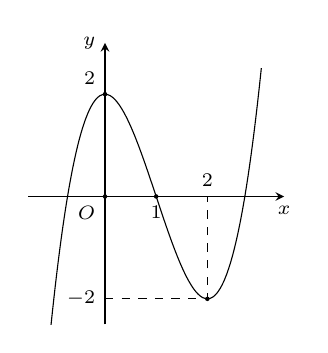
\begin{tikzpicture}[>=stealth,x=1cm,y=1cm,scale=.65]
			\def\a{1} 
			 \def\b{-3}
			 \def\c{0}
			\def\d{2} 
			\draw[->]  (-1.5,0) -- (3.5,0) node[below]{\scriptsize $x$};
			\draw[->] (0,-2.5) -- (0,3)  node[left] {\scriptsize $y$};
			\draw[dashed] (0,0) node[below  left]{\scriptsize $O$}
				(0,2)  node[above left]{\scriptsize $2$}
				 (1,0) node[below]{\scriptsize $1$}
				(0,-2)  node[left]{\scriptsize $-2$}-|(2,0) node[above]{\scriptsize $2$};
			\clip (-1.5,-2.5) rectangle (3.5,2.5); 
			\draw[samples=150,smooth,domain=-5:5]  plot (\x,{\a*(\x)^3+(\b)*(\x)^2+(\c)*\x+(\d)});
			\fill (0,0) circle  (1.25pt);
			\fill  (1,0) circle (1.25pt);
			\fill (2,-2) circle (1.25pt); 
			\fill  (0,2) circle (1.25pt);
		\end{tikzpicture}
		 }
	 \loigiai{
		 Hàm số đạt cực tiểu tại $x=2$.
	} 
\end{ex}

% nguồn: Phan1_Lop_12_Dai_so_Chuong_1
\begin{ex}%[2D1N2-2]%[ma:1a536494]
	\immini{Cho hàm số $y=f(x)$ có đồ thị như hình bên. Phát biểu nào sau đây là đúng? 
	\choice 
		{$y_{\text{ CT}}=1,y_{\text{  CĐ}}=2$}
		{$y_{\text{  CT}}=2,y_{\text{ CĐ}}=-1$}
		 {$y_{\text{ CT}}=-2,y_{\text{ CĐ}}=2$}
		{\True $y_{\text{  CT}}=2,y_{\text{ CĐ}}=-2$}
		}{\resizebox{!}{5cm}{ 
		\begin{tikzpicture}[scale=0.5,>=stealth,line join=round,line cap=round]
			\draw[->] (-6,0)--(6,0) node[below]{$x$}; 
			\draw[->]  (0,-6)--(0,6) node[left]{$y$};
			\draw[samples=100,domain=-5:-0.175]  plot (\x,{(\x)+1/(\x)});
			\draw[samples=100,domain=0.18:5]  plot (\x,{(\x)+1/(\x)});
			 \draw[samples=100,domain=-5:5] plot (\x,{(\x)});
			\draw (0,0) node[below  right]{$O$};
			 \draw[dashed]
				(-1,0)  node[below left]{$-1$}
				(0,-2)  node[right]{$-2$}
				(0,2) node[above left]{$2$} 
				(1,0)  node[below right]{$1$}
				 (1,0)--(1,2)--(0,2)
				 (-1,0)--(-1,-2)--(0,-2);
			\fill (1,2)  circle (1pt)
				 (-1,-2) circle (1pt)
				(0,0) circle (1pt); 
		\end{tikzpicture}
		 }
		 }
	\loigiai{ 
		Dựa vào đồ thị ta thấy hàm số có $y_{\text{ CT}}=2, y_{\text{ CĐ}}=-2$. 
	} 
\end{ex}

% nguồn: Phan1_Lop_12_Dai_so_Chuong_1
\begin{ex}%[2D1N2-2]%[ma:b2ba77d1]
	 \immini{Cho hàm số có đồ thị như hình bên.
	 Khẳng định nào \textbf{sai}?
	 \choice
		{Hàm số có một cực tiểu tại  $x=\dfrac{3}{4}$ và đạt cực đại tại $x=0$}
		{Giá trị cực đại $y=-1$ và giá trị cực tiểu $y=-\dfrac{113}{32}$} 
		{Hàm số  có một cực tiểu tại $x=-\dfrac{3}{4}$}
		{\True Hàm số có một cực đại tại $x=-\dfrac{3}{4}$} 
		}{ 
		\begin{tikzpicture}[line cap=round,>=stealth,scale=0.9]
			\tikzset{ethicknode/.style={scale=0.8}} 
			\draw[->] (-1.75,0)--(1.75,0) node[below  left] {$x$};
			\draw[->] (0,-4.531)--(0,1) node[below left] {$y$}; 
			\draw  (0,0) node [below left] {$O$};
			\draw[dashed,thin](-0.75,0) node[above] {$-\dfrac{3}{4}$}--(-0.75,-3.531)--(0.75,-3.531)--(0.75,0) node[above] {$\dfrac{3}{4}$}; 
			\path (0,-3.531) node[below left] {$-\dfrac{113}{32}$} 
				(0,-1)  node[above right]{$-1$};
			\begin{scope}
				 \clip (-1.75,-4.431) rectangle (1.75,0.9);
				\draw[samples=200,domain=-1.65:1.65,smooth,variable=\x] plot  (\x,{8*((\x)^4)-9*((\x)^2)-1});
			\end{scope}
		\end{tikzpicture}
		} 
	 \loigiai{
		Dựa vào đồ  thị ta thấy, hàm số đạt cực đại tại $x=0, y_{\text{ CĐ}}=-1$.\\
		Hàm số đạt cực tiểu tại $x=-\dfrac{3}{4}$  và $x=\dfrac{3}{4}$, $y_{\text{ CT}}=-\dfrac{113}{32}$.
	 }
\end{ex}

% nguồn: Phan1_Lop_12_Dai_so_Chuong_1
\begin{ex}%[2D1N2-2]%[ma:c2eb3686]
	Cho hàm số $y=f(x)$ xác định trên $\mathbb{R}$ và có bảng biến thiên như  hình vẽ sau
	\begin{center}
		
\begin{tikzpicture}
			\tkzTabInit[nocadre=false,lgt=1,espcl=2] 
				 {$x$ /0.6,$y'$ /0.7,$y$ /1.7}
				 {$-\infty$,$10$,$12$,$+\infty$}
			\tkzTabLine{,+,0,-,0,+,} 
			\tkzTabVar{-/$-\infty$,+/$-3$,-/ $3$  /,+/$-\infty$ /}
		\end{tikzpicture}
	\end{center}
	Hàm số  $y=f(x)$ đạt cực đại tại
	\choice 
		 {\True $x=10$}
		{$x=8$} 
		{$x=12$} 
		{$x=17$} 
	\loigiai{ 
		Dựa vào bảng biến thiên ta thấy  hàm số đạt cực đại tại $x=10$.
	} 
\end{ex}

% nguồn: Phan1_Lop_12_Dai_so_Chuong_1
\begin{ex}%[2D1N2-2]%[ma:b3546e0c]
	Cho hàm số $y=f(x)$ có bảng xét dấu của đạo hàm như hình bên. Số điểm cực tiểu của hàm số $y=f(x)$  là
	\begin{center}
		
\begin{tikzpicture}[>=stealth,scale=0.9]
			\tkzTabInit[lgt=2,espcl=2] 
				 {$x$/0.8,$f^{\prime}
				(x)$/0.8} 
				{$-\infty$,$-3$,$1$,$3$,$+\infty$} 
			\tkzTabLine{,-,0,+,0,-,0,+,} 
		\end{tikzpicture}
	\end{center}
	 \choice
		 {$3$}
		{$4$} 
		{\True $2$} 
		{$1$} 
	 \loigiai{
		Hàm số đạt cực tiểu tại điểm $x=-3$ và $x=3$ nên số điểm cực tiểu  của hàm số là $2$.
	 }
\end{ex}

% nguồn: Phan1_Lop_12_Dai_so_Chuong_1
\begin{ex}%[2D1N2-2]%[ma:cf3765aa]
	 Hàm số $y=f\left( x \right)$ xác định, liên tục trên $\mathbb{R}$ và có bảng biến thiên như hình vẽ bên dưới. Khẳng định nào sau đây đúng?
	\begin{center}
		
\begin{tikzpicture}[>=stealth]
			\tkzTabInit[nocadre=true,lgt=1.2,espcl=2,deltacl=0.5]{$x$/.7,$f'(x)$/.7,$f  (x)$/2}
				{$-\infty$,$0$,$1$,$2$,$+\infty$} 
			\tkzTabLine{,-,d,+,$0$,+,$0$,-,} 
			\tkzTabVar{+/$+\infty$,-/$0$,R/,+/$1$,-/$0$} 
		\end{tikzpicture}
	\end{center}
	\choice 
		{Hàm số  đạt cực tiểu tại $x=-1$}
		{Hàm số có giá trị lớn nhất bằng $1$  và giá trị nhỏ nhất bằng $-1$}
		{\True Hàm số có đúng hai điểm  cực trị}
		{Hàm số đạt cực đại tại $x=0$, $x=1$ và đạt cực  tiểu tại $x=2$}
	\loigiai{Dựa vào bảng biến thiên ta có hàm số có đúng hai cực trị tại $x=0$ và  $x=2$.}
\end{ex}

% nguồn: Phan1_Lop_12_Dai_so_Chuong_1
\begin{ex}%[2D1N2-2]%[ma:36a07538]
	 \immini{
	Cho hàm số $y=ax^3+bx^2+cx+d \,(a,b,c,d\in \mathbb{R})$ có đồ thị là đường cong trong hình bên. Giá trị cực đại của hàm số đã cho  bằng
	 \choice
		{$0$} 
		 {\True $3$}
		{$1$} 
		 {$-1$}
		 }
		 {
		\begin{tikzpicture}[>=stealth,scale=0.8,font=\footnotesize]
			\draw[->] (-2.5,0)--(3,0) node[below]  {$x$};
			\draw[->] (0,-2)--(0,4) node[left] {$y$}; 
			\draw[domain=-2:2,samples=100]  plot (\x,{-(\x)^3+3*\x+1});
			\draw (0,0) node[below right=-0.1]  {$O$} circle (1.2pt);
			\draw (1,0) node[above right]  {$1$} circle (1.2pt);
			 \draw (-1,0) node[above] {$-1$} circle (1.2pt);
			\draw (0,-1) node[right] {$-1$} circle (1.2pt); 
			\draw  (0,1) node[right] {$1$} circle (1.2pt);
			\draw (0,3) node[left] {$3$}  circle (1.2pt);
			\draw[dashed]  (1,0)--(1,3)--(0,3)
				(-1,0)--(-1,-1)--(0,-1); 
		\end{tikzpicture}
		 }
	\loigiai{ 
	Từ đồ thị hàm số, giá  trị cực đại của hàm số đã cho bằng $3$.}
\end{ex}

% nguồn: Phan1_Lop_12_Dai_so_Chuong_1
\begin{ex}%[2D1N2-2]%[ma:b1f28748]
	Cho hàm số có bảng biến  thiên như \textit{Hình 2}. Giá trị cực tiểu của hàm số đã cho là
	\choice 
		{$-2$} 
		{\True $ -1$} 
		{$  0$}
		 {$3$}
	\loigiai{ 
		Từ bảng biến thiên ta có giá trị cực tiểu của hàm số đã cho là $y=-1$. 
	 }
\end{ex}

% nguồn: Phan1_Lop_12_Dai_so_Chuong_1
\begin{ex}%[2D1N2-2]%[ma:439382a1]
	Cho hàm số $y=f(x)$ có đồ thị như \textit{Hình 1}. Điểm cực tiểu của hàm số đã cho  là
	\choice 
		 {$-1$}
		{\True $ 1$} 
		{$ 0$} 
		{$4$} 
	\loigiai{ 
	Từ đồ thị  ta có điểm cực tiểu của hàm số đã cho là $x=1$.}
\end{ex}

% nguồn: Phan1_Lop_12_Dai_so_Chuong_1
\begin{ex}%[2D1N2-2]%[ma:06e77e60]
	\immini{Cho hàm  số $y=ax^4+bx^3+cx^2+dx+e, (a, b,c,d,e \in \mathbb{R})$
	có đồ  thị như hình bên. Số điểm cực trị của hàm số là
	 \choice
		{$0$} 
		{$1$} 
		 {$2$}
		{\True $3$}} 
		 {
		\begin{tikzpicture}[>=stealth,scale=0.8]
			\draw[->]  (-2.5,0)--(2.5,0) node[below]{$x$};
			 \draw[->] (0,-1.5)--(0,2.2) node[left]{$y$};
			\begin{scope}
				\clip (-2.3,-2.5)  rectangle (2.3,2);
				\draw[samples=100,domain=2:-2] plot (\x,{(\x)^4-2*(\x)^2}); 
			\end{scope}
			\draw (0,0)  node[above left]{$O$};
		\end{tikzpicture}
		} 
	\loigiai{ 
		Dựa vào đồ thị hàm số ta suy ra  số điểm cực trị của hàm số là $3$.
	} 
\end{ex}

% nguồn: Phan1_Lop_12_Dai_so_Chuong_1
\begin{ex}%[2D1N2-2]%[ma:d4f134b2]
	\immini{Cho hàm số $y=f(x)$ liên tục trên $\mathbb{R}$ và có đồ thị như hình bên. Phát  biểu nào sau đây là đúng?
	\choice 
		{$x_{\text{ CT}}=-1$, $x_{\text{  CĐ}}=1$}
		{$x_{\text{ CT}}=-3$, $x_{\text{ CĐ}}=1$} 
		{$x_{\text{ CT}}=1$, $x_{\text{  CĐ}}=-3$}
		{\True $x_{\text{ CT}}=1$, $x_{\text{ CĐ}}=-1$}} 
		{\resizebox{!}{4cm}{\begin{tikzpicture}[line join=round,line cap=round,>=stealth]
		\draw[->] (-3.1,0)--(3.1,0) node[below left]  {$x$};
		\draw[->] (0,-3.6)--(0,2.5) node[below left] {$y$}; 
		\fill (0,0) circle (1pt) node [below  right] {$O$};
		\draw[dashed,thin](-1,0)  node[below]{$-1$}--(-1,1)--(0,1) node[right]{$1$};
		\draw[dashed,thin](1,0) node[above]{$1$}--(1,-3)--(0,-3)  node[left]{$-3$};
		\begin{scope}
			\clip (-3,-3.5)  rectangle (2.5,2);
			\draw[samples=100,domain=-4:4,smooth,variable=\x] plot  (\x,{((\x)^3)+0*((\x)^2)+-3*(\x)-1});
		\end{scope}
		 \fill (-1,1) circle (1pt)
			(0,-1) circle  (1pt)
			(1,-3) circle  (1pt);
	\end{tikzpicture}
		 }
		 }
	\loigiai{ 
		Dựa  vào đồ thị ta thấy hàm số có $x_{\text{ CT}}=1$, $x_{\text{ CĐ}}=-1$.
	} 
\end{ex}

% nguồn: Phan1_Lop_12_Dai_so_Chuong_1
\begin{ex}%[2D1N2-2]%[ma:8d339d27]
	Cho hàm số $f(x)$ có bảng biến  thiên như hình sau.
	\begin{center}
		
\begin{tikzpicture}[scale=1,font=\footnotesize,line join=round,line cap=round,>=stealth]
			\tkzTabInit[nocadre=True,lgt=1,espcl=3,deltacl=0.5] 
				{$x$/.7,$f'(x)$/.7,$f  (x)$/2}
				 {$-\infty$,$-1$,$0$,$1$,$+\infty$}
			 \tkzTabLine{,+,0,-,d,-,0,+,}
			 \tkzTabVar{-/$-\infty$,+/$-2$,-D+/$-\infty$/$+\infty$,-/$2$,+/$+\infty$}
		\end{tikzpicture}
	\end{center}
	Điểm cực đại của hàm  số là
	 \choice
		 {\True $x_{\text{ CĐ}}=-1$}
		{$x_{\text{ CĐ}}=1$} 
		{$x_{\text{  CĐ}}=-2$}
		 {$x_{\text{ CĐ}}=2$}
	 \loigiai{
		Từ bảng  biến thiên suy ra hàm số đạt cực đại tại $x_{\text{ CĐ}}=-1$.
	} 
\end{ex}

% nguồn: Phan1_Lop_12_Dai_so_Chuong_1
\begin{ex}%[2D1N2-2]%[ma:0b04e512]
	Cho hàm số $f(x)$ có bảng biến thiên như  sau:
	\begin{center}
		
\begin{tikzpicture}
			\tkzTabInit[nocadre=false,lgt=1.3,espcl=2.5]{$x$ /1,$f'(x)$  /1,$f (x)$ /2}{$-\infty$,$-1$,$2$,$+\infty$}
			\tkzTabLine{,-,$0$,+,$0$,-,} 
			 \tkzTabVar{+/ $+\infty$,-/$-2$,+/$3$,-/$-\infty$}
		\end{tikzpicture}
	\end{center}
	Giá trị cực  đại của hàm số đã cho là
	 \choice
		{\True  $3$}
		 {$-2$}
		 {$-1$}
		{$2$} 
	\loigiai{ 
	Dựa vào  bảng biến thiên ta suy ra giá trị cực đại của hàm số đã cho là $3$.}
\end{ex}

% nguồn: Phan1_Lop_12_Dai_so_Chuong_1
\begin{ex}%[2D1N2-2]%[ma:5c666585]
	Cho hàm số $y=f(x)$ liên tục trên $ \mathbb{R}$ và có bảng xét dấu của $f'(x)$ như sau:\\ 
	\begin{center}
		\resizebox{0.8\linewidth}{!}{
\begin{tikzpicture}
		\tkzTabInit[nocadre,espcl=2.5,lgt=1.5] 
			 {$x$/0.7,$f'(x)$/0.7}
			{$-\infty$,$-1$,$0$,$1$,$2$,$+\infty$} 
		 \tkzTabLine{,+,0,-,d,+,0,+,0,-,}
	\end{tikzpicture}
		} 
	\end{center}
	 Số điểm cực trị của hàm số là:
	\choice 
		{$1$} 
		{$2$} 
		{\True  $3$}
		 {$4$}
	\loigiai{ 
	Hàm số đạt cực trị tại  $x=-1$, $x=0$ và $x=2$.}
\end{ex}

% nguồn: Phan1_Lop_12_Dai_so_Chuong_1
\begin{ex}%[2D1H2-2]%[ma:af4b716b]
	 Cho hàm số $y=f(x)$ xác định và liên tục trên $\mathbb{R}$ có bảng biến thiên như hình vẽ. Gía trị nhỏ nhất của hàm số trên khoảng $(-2;+\infty)$ bằng?
	\begin{center}
		
\begin{tikzpicture}
			 \tkzTabInit[nocadre,lgt=1,espcl=2.3]
				{$x$ /0.7,$y'$ /0.7,$y$  /2}
				 {$-\infty$,$-2$,$5$,$+\infty$}
			 \tkzTabLine{,+,0,-,0,+,}
			\tkzTabVar{-/$-\infty$,+/ $1$,-/ $0$  /,+/$+\infty$ /}
		\end{tikzpicture}
	\end{center}
	\choice 
		{\True $0$} 
		 {$1$}
		{$-2$} 
		 {$5$}
	 \loigiai{
		Dựa vào  bảng biến thiên trên khoảng $(-2;+\infty)$
		ta  có giá trị nhỏ nhất là $0$ tại $x=5$.
	 }
\end{ex}

% nguồn: Phan1_Lop_12_Dai_so_Chuong_1
\begin{ex}%[2D1H2-2]%[ma:2da6d05a]
	Cho hàm số $y=f(x)$ có đạo hàm trên $\mathbb{R}$ có bảng xét  dấu của đạo hàm như sau:
	\begin{center}
		\resizebox{0.8\linewidth}{!}{
\begin{tikzpicture}
		\tkzTabInit[nocadre,lgt=1.3]{$x$ /1,$f'(x)$  /1}{$-\infty$,$1$,$2$,$3$,$+\infty$}
		 \tkzTabLine{,+,$0$,-,$0$,+,$0$,-,}
	\end{tikzpicture}
		 }
	\end{center}
	Phát biểu nào sau đây là đúng? 
	\choice 
		{Hàm số $y=f(x)$ không có  điểm cực tiểu}
		{\True Hàm số $y=f(x)$ có đúng một  điểm cực tiểu}
		{Hàm số $y=f(x)$ có đúng hai điểm cực  tiểu}
		{Hàm số  $y=f(x)$ có đúng ba điểm cực tiểu}
	\loigiai{ 
		Từ bảng xét dấu của hàm  số $f(x)$ các định trên $\mathbb{R}$, ta có bảng biến thiên sau
		\begin{center}
			
\begin{tikzpicture}
				\tkzTabInit[nocadre,lgt=1.3,espcl=2.5]{$x$ /1,$f'(x)$ /1,$f  (x)$ /2}{$-\infty$,$1$,$2$,$3$,$+\infty$}
				\tkzTabLine{,+,$0$,-,$0$,+,$0$,-,} 
				\tkzTabVar{-/ $ $,+/$ $,-/$ $,+/$ $,-/$ $} 
			\end{tikzpicture}
		\end{center}
		Ta suy ra  hàm số $y=f(x)$ có đúng một điểm cực tiểu.
	} 
\end{ex}

% nguồn: Phan1_Lop_12_Dai_so_Chuong_1
\begin{ex}%[2D1H2-2]%[ma:0ade406a]
	\immini{Cho hàm số $y=f(x)$ có đạo hàm trên $\mathbb{R}$ và hàm số $y=f'(x)$ có đồ thị như hình  bên. Khẳng định nào sau đây \textbf{đúng}?
	\choice 
		{Hàm số  $y=f(x)$ đồng biến trên $(-\infty;1)$}
		{\True Hàm số  $y=f(x)$ nghịch biến trên $(2;4)$}
		{Hàm số $y=f(x)$ đạt cực  tiểu tại $x=3$}
		{Hàm số $y=f(x)$ đạt cực đại tại $x=4$}} 
		{ 
		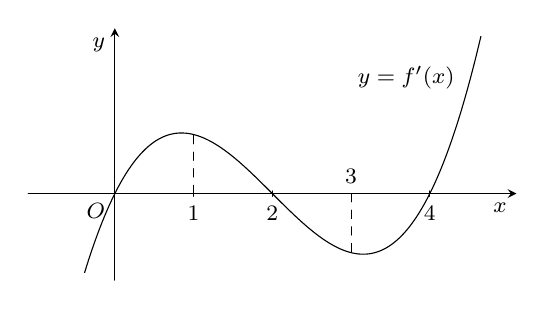
\begin{tikzpicture}[scale=1,line join=round,font=\footnotesize,line cap=round,>=stealth]
			 \tikzset{ethicknode/.style={scale=0.9}}
			\draw[->] (-1.1,0)--(5.1,0) node[below  left] {$x$};
			\draw[->] (0,-1.1)--(0,2.1) node[below left] {$y$}; 
			\draw  (0,0) node [below left] {$O$};
			\foreach \x/\nx  in {1/1,2/2,4/4}
			\draw[thin] (\x,1pt)--(\x,-1pt) node  [below] {$\nx$};
			\begin{scope}
				\clip (-1,-1) rectangle (5,2); 
				\draw[samples=200,domain=-1:5,smooth,variable=\x] plot  (\x,{0.25*((\x)^3)-1.5*((\x)^2)+2*(\x)});
				 \draw[dashed] (1,0)--(1,0.75);
				\draw[dashed] (3,0)--(3,-0.75); 
				\path  (3,0) node[above]{$3$};
				\path (3.7,1.2)  node[above]{$y=f'(x)$};
			\end{scope}
		\end{tikzpicture}
		 }
	 \loigiai{
		Từ đồ thị  hàm số $y=f'(x)$ ta thấy $f'(x)<0$ trên các khoảng $(-\infty;0)$ và $(2;4)$.\\
		Do đó  hàm số $y=f(x)$ nghịch biến trên các khoảng $(-\infty;0)$ và $(2;4)$.
	} 
\end{ex}

% nguồn: Phan1_Lop_12_Dai_so_Chuong_1
\begin{ex}%[2D1H2-2]%[ma:61dcb27a]
	Cho hàm số $y=f(x)$ có đạo hàm trên $\mathbb{R}$ và có bảng xét dấu của  đạo hàm như sau:
	\begin{center}
		
\begin{tikzpicture}
			\tkzTabInit[nocadre,lgt=1.3]{$x$ /1,$f'(x)$ /1}{$-\infty$,$1$,$8$,$+\infty$} 
			\tkzTabLine{,+,$0$,-,$0$,+,} 
		\end{tikzpicture}
	\end{center}
	Phát biểu nào sau đây là  đúng?
	 \choice
		 {Hàm số có điểm cực tiểu là $x_1=1$ và có điểm cực đại là $x_2=8$}
		{\True Hàm số có điểm cực đại là  $x_1=1$ và có điểm cực tiểu là $x_2=8$}
		{Hàm số có hai điểm cực  tiểu là $x_1=1$ và $x_2=8$}
		{Hàm số có hai điểm cực đại là $x_1=1$ và  $x_2=8$}
	 \loigiai{
		Từ bảng xét dấu của hàm số  $f(x)$ các định trên $\mathbb{R}$, ta có bảng biến thiên sau
		\begin{center}
			
\begin{tikzpicture}
				\tkzTabInit[nocadre,lgt=1.3,espcl=2.5]{$x$ /1,$f'(x)$ /1,$f (x)$ /2}{$-\infty$,$1$,$8$,$+\infty$} 
				\tkzTabLine{,+,$0$,-,$0$,+,} 
				\tkzTabVar{-/  $ $,+/$ $,-/$ $,+/$ $}
			\end{tikzpicture}
		\end{center}
		Ta suy ra hàm số có điểm cực đại là $x_1=1$ và có điểm cực  tiểu là $x_2=8$.
	} 
\end{ex}

% nguồn: Phan1_Lop_12_Dai_so_Chuong_1
\begin{ex}%[2D1H2-2]%[ma:e4188558]
	Cho hàm số $y=f(x)$ có  đạo hàm trên $\mathbb{R}$ có bảng xét dấu của đạo hàm như sau:
	\begin{center}
		\resizebox{0.8\linewidth}{!}{
\begin{tikzpicture}
		\tkzTabInit[nocadre,lgt=1.3]{$x$ /1,$f'(x)$  /1}{$-\infty$,$1$,$2$,$3$,$+\infty$}
		\tkzTabLine{,-,$0$,+,$0$,-,$0$,+,} 
	\end{tikzpicture}
		 }
	\end{center}
	Phát biểu nào sau  đây là đúng?
	 \choice
		{Hàm  số $y=f(x)$ không có điểm cực tiểu}
		{Hàm số $y=f(x)$ có đúng một điểm cực tiểu} 
		{\True Hàm số $y=f(x)$ có đúng hai  điểm cực tiểu}
		{Hàm số $y=f(x)$ có  đúng ba điểm cực tiểu}
	\loigiai{ 
		Từ bảng xét dấu của hàm số $f(x)$ các định trên $\mathbb{R}$, ta có bảng  biến thiên sau
		\begin{center}
			\resizebox{0.8\linewidth}{!}{
\begin{tikzpicture}
		\tkzTabInit[nocadre,lgt=1.3,espcl=2.5]{$x$ /1,$f'(x)$ /1,$f (x)$ /2}{$-\infty$,$1$,$2$,$3$,$+\infty$} 
		\tkzTabLine{,-,$0$,+,$0$,-,$0$,+,} 
		\tkzTabVar{+/ $ $,-/$  $,+/$ $,-/$ $,+/$ $}
	\end{tikzpicture}
			} 
		\end{center}
		 Ta suy ra hàm số $y=f(x)$ có đúng hai điểm cực tiểu.
	 }
\end{ex}

% nguồn: Phan1_Lop_12_Dai_so_Chuong_1
\begin{ex}%[2D1H2-2]%[ma:70832669]
	\immini{Cho hàm số  $y=f(x)$ có đồ thị như hình vẽ. Điểm cực đại của đồ thị hàm số là
	 \choice
		{$x=2$} 
		{$x=0$} 
		{\True$(2;-3)$} 
		{$(0;1)$}}{ 
		\begin{tikzpicture}[>=stealth,x=1cm,y=1cm,scale=.65]
			\def\a{-1} 
			\def\b{1} 
			 \def\c{-1}
			\def\d{1} 
			\def\e{-1} 
			 \draw[->] (-4,0) -- (5,0) node[below] {\scriptsize $x$};
			\draw[->]  (0,-5) -- (0,4) node[left] {\scriptsize $y$};
			\draw[dashed] (0,0)  node[below left]{\scriptsize $O$}
				(0,1)  node[above left]{\scriptsize $1$}
				(1,0) node[below right]{\scriptsize $1$} 
				(2,0) node[above]{\scriptsize $2$}|-(0,-3)  node[left]{\scriptsize $-3$}
				(0,-1)  node[left]{\scriptsize $-1$}--(1,-1);
			\draw[dashed,blue]  (1,-5)--(1,4)
				(-4,4)--(5,-5); 
			\clip  (-4,-5) rectangle (5,4);
			\pgfmathsetmacro{\can}{-(\e)/(\d)} 
			\draw[samples=150,smooth,domain=-5:{\can-.1}] plot (\x,{(\a*(\x)^2+(\b)*\x+\c)/(\d*\x+(\e))}); 
			 \draw[samples=150,smooth,domain={\can+.1}:5] plot (\x,{(\a*(\x)^2+(\b)*\x+\c)/(\d*\x+(\e))});
			\fill  (0,0) circle (1.25pt);
			\fill (2,-3) circle (1.25pt); 
			 \fill (1,-1) circle (1.25pt);
			\fill  (0,1) circle (1.25pt);
		\end{tikzpicture}
		 }
	 \loigiai{
		Nhìn vào đồ thị hàm số  $y=f(x)$, ta có điểm cực đại của đồ thị hàm số là $(2;-3)$.
	 }
\end{ex}

% nguồn: Phan1_Lop_12_Dai_so_Chuong_1
\begin{ex}%[2D1Y2-2]%[ma:23ad91db]
	Cho hàm số $y=f(x)$ liên tục trên $\mathbb{R}$ và có bảng xét  dấu đạo hàm như sau:
	\begin{center}
		
\begin{tikzpicture}
			\tkzTabInit[nocadre=true,lgt=2,espcl=2,deltacl=0.5] 
				{$x$/1,$f'(x)$/1} 
				 {$-\infty$,$0$,$1$,$2$,$4$,$+\infty$}
			 \tkzTabLine{,-,0,+,d,-,0,+,0,+}
		\end{tikzpicture}
	\end{center}
	Khẳng định nào sau đây đúng? 
	 \choice
		{\True Hàm số có $2$ điểm  cực tiểu và $1$ điểm cực đại}
		 {Hàm số có $2$ điểm cực đại và $2$ điểm cực tiểu}
		{Hàm số có $2$ điểm cực tiểu và  không có điểm cực đại}
		{Hàm số có $1$ điểm  cực tiểu và $2$ điểm cực đại}
	 \loigiai{
	Dựa vào bảng biến thiên, hàm số có $2$ điểm  cực tiểu và $1$ điểm cực đại.}
\end{ex}


%%%%%%%%%%%%%%%% ĐÚNG/SAI %%%%%%%%%%%%%%%%

% nguồn: Phan1_Lop_12_Dai_so_Chuong_1
\begin{ex}%[2D1H2-2]%[ma:16cdede5]
	Đạo hàm $f'(x)$ của hàm số $y=f(x)$ có đồ thị như hình  vẽ.
	\begin{center}
		\begin{tikzpicture}[scale=0.7,font=\footnotesize,line join=round,line cap=round,>=stealth]
			\def\a{0.125} \def\b{-0.625} \def\c{0.25}  \def\d{1}
			\def\xt{-3}  \def\xp{6} \def\yt{2.5} \def\yd{-3}
			\draw[->] (\xt,0)--(\xp,0) node [below]{$x$}; 
			\draw[->] (0,\yd)--(0,\yt) node  [left]{$y$};
			\node at (0,0)  [below right]{$O$};
			 \clip (\xt+0.1,\yd-1) rectangle (\xp-0.1,\yt-0.1);
			\draw[smooth,samples=200,domain=-2:5] plot (\x,{\a*(\x)^3+\b*(\x)^2+\c*(\x)+\d}) node [below  left]{$y=f'(x)$};
			\draw[dashed] (-2,0) node [below left]{$-2$} --  (-2,-3)
				(5,0) node [below]{$5$} -- (5,2.25); 
			\fill (-1,0) circle (1.5pt)  node[below right]{$-1$}
				(1,0)  circle (1.5pt) node[below]{$1$}
				(3,0)  circle (1.5pt) node[above]{$3$}
				(2,0)  circle (1.5pt) node[below left]{$2$}
				(4,0) circle (1.5pt) node[below right]{$4$}; 
		\end{tikzpicture}
	\end{center}
	 \choiceTF
		{Hàm số đạt cực tiểu  tại $x=-1$ và $x=3$}
		{\True  Hàm số đồng biến trên $(-1;2)$ và $(4;5)$}
		{Hàm số nghịch  biến trên $(0; 3)$}
		 {\True $f(2)>f(3)>f(4)$}
	 \loigiai{
		Từ đồ thị ta  thấy $f'(x)=0 \Leftrightarrow \hoac{& x=-1\\ & x=2\\ & x=4.}$\\
		Ta có bảng biến thiên như  sau
		\begin{center}
			
\begin{tikzpicture}
				\tkzTabInit[nocadre=true,lgt=1.2,espcl=2.5,deltacl=0.6] 
					{$x$  /0.6,$f'(x)$ /0.6,$f (x)$ /2}
					 {$-2$,$-1$,$2$,$4$,$5$}
				\tkzTabLine{,-,$0$,+,$0$,-,$0$,+,} 
				 \tkzTabVar{+/,-/,+/,-/,+/}
			\end{tikzpicture}
		\end{center}
		Từ  bảng biến thiên suy ra
		\begin{itemchoice}
			\itemch Hàm số đạt cực  tiểu tại $x=-1$, $x=4$.
			 \itemch Hàm số đồng biến trên $(-1;2)$ và $(4;5)$.
			 \itemch Hàm số nghịch biến trên $(-2;-1)$ và $(2;4)$.
			\itemch Hàm số $f(x)$ nghịch  biến trên khoảng $(2; 4)$, ta có $2<3<4\Rightarrow f(2)>f(3)>f(4)$.
		\end{itemchoice}
	 }
\end{ex}

% nguồn: Phan1_Lop_12_Dai_so_Chuong_1
\begin{ex}%[2D1H2-2]%[ma:20dbeccc]
	Cho hàm  số $y=f(x)$ có bảng biến thiên như hình vẽ
	\begin{center}
		\begin{tikzpicture}[>=stealth,scale=0.8]
			 \tkzTabInit[lgt=2,espcl=2]
				 {$x$/0.8,$y^{\prime}$/0.8,$y$/3}
				 {$-\infty$,$-2$,$0$,$1$,$+\infty$}
			\tkzTabLine{,-,0,+,d,+,0,-,} 
			 \path
				 (N12) node[shift={(0,-0.3)}](A){$+\infty$}
				(N23)  node[shift={(0,0.3)}](B){$-1$}
				(N32)  node[shift={(-0.5,-0.3)}](C){$2$}
				 (N33) node[shift={(0.5,0.3)}](D){$-\infty$}
				(N42) node[shift={(0,-0.3)}](E){$2$} 
				(N53)  node[shift={(0,0.3)}](F){$-\infty$};
			\foreach\X/\Y  in{A/B,B/C,D/E,E/F}\draw[->](\X)--(\Y);
			\draw[double,double  distance=2pt](N32)--(N33);
		\end{tikzpicture}
	\end{center}
	 \choiceTF
		{\True Giá trị  cực tiểu của hàm số bằng $1$}
		{\True Hàm số đạt cực  tiểu tại $x=-2$}
		{Giá trị cực đại của  hàm số bằng $2$}
		{\True  Hàm số đạt cực đại tại $x=0$ và $x=1$}
	 \loigiai{
		Từ bảng biến thiên ta thấy hàm số $y=f(x)$ có đạo hàm đổi dấu từ $(-)$ sang $(+)$ khi  $x$ đi qua $x_1 = -2 \Rightarrow y_{CT} = -1$.\\
		Do đó mệnh đề  \lq\lq Giá trị cực tiểu của hàm số bằng bằng $-1$\rq\rq~ và mệnh đề \lq\lq~Hàm số đạt cực tiểu tại $x=-2$\rq\rq~ là mệnh đề đúng.\\
		Hàm số $y=f(x)$  có đạo hàm đổi dấu từ $(+)$ sang $(-)$ khi $x$ đi qua $x_2=1 \Rightarrow y_{CD}=2$ do đó mệnh đề \lq\lq Giá trị cực đại của hàm số bằng $2$\rq\rq~là mệnh đề đúng.
		\begin{itemchoice}
			\itemch Giá trị cực  tiểu của hàm số bằng $1$.
			\itemch Hàm số đạt cực tiểu tại $x=-2$. 
			\itemch Giá trị cực đại của hàm số bằng $2$. 
			\itemch Hàm số đạt cực  đại tại $x=1$.
		\end{itemchoice}
	} 
\end{ex}

% nguồn: Phan1_Lop_12_Dai_so_Chuong_1
\begin{ex}%[2D1H2-2]%[ma:5c77de6e]
	Cho hàm số $y=f(x)$ liên tục trên $\mathbb{R}$  thỏa mãn $f(1) \leq f(x) \leq f(-1)$, $\forall x \in \mathbb{R}$.
	\choiceTF 
		{\True Giá trị  nhỏ nhất của hàm số trên $\mathbb{R}$ là $f(1)$}
		{\True Giá trị lớn nhất của hàm số trên $\mathbb{R}$ là  $f(-1)$}
		{Điểm cực tiểu của hàm số là  $x_\text{ CT}=-1$}
		 {Điểm cực đại của hàm số là $x_\text{ CĐ}=1$}
	\loigiai{ 
		\begin{itemchoice}
			\itemch {\bf Đúng}.\\ 
			Hàm số có giá trị  lớn nhất là $f(-1)$ tại $x=-1$.
			\itemch {\bf Đúng}.\\ 
			Hàm số có giá  trị nhỏ nhất là $f(1)$ tại $x=1$.
			\itemch {\bf Sai}.\\ 
			Vì lân  cận $x=-1$ thì $f(-1)$ lớn nhất.
			\itemch {\bf  Sai}.\\
			 Vì lân cận $x=1$ thì $f(1)$ nhỏ nhất.
		\end{itemchoice}
	 }
\end{ex}

% nguồn: Phan1_Lop_12_Dai_so_Chuong_1
\begin{ex}%[2D1H2-2]%[ma:d4d84d98]
	 \immini
	{Cho hàm số bậc ba $y = f(x)$ có đồ thị $(C)$ như hình  vẽ
	 \choiceTF
		{\True Hàm  số đạt cực đại tại điểm $x = -1$}
		 {\True Hàm số $y = f(x)$ đồng biến trên khoảng $(1; +\infty)$}
		{Hai điểm cực trị của đồ  thị hàm số cùng với gốc tọa độ tạo thành tam giác có diện tích bằng $2$}
		{Khoảng cách giữa hai điểm cực trị của  đồ thị hàm số bằng $3\sqrt{5}$}}
		{\resizebox{!}{5cm}{\begin{tikzpicture}
		\draw[->] (-3,0) -- (3,0)  node[right]{$x$};
		\draw[->] (0,-2) -- (0,3.5) node[left]{$y$}; 
		\node[below left] at  (0,0) {$O$};
		 \node[above] at (1,0) {$1$};
		\node[left]  at (0,1) {$1$};
		\node[right] at (0,3) {$3$}; 
		\node[below left] at (-1,0)  {$-1$};
		\node[left] at  (0,-1) {$-1$};
		\draw[domain=-2.1:2.1,samples=100] plot  (\x,{(\x*\x*\x)-(3*\x)+1});
		 \draw[dashed] (-1,0) -- (-1,3);
		\draw[dashed] (1,0) --  (1,-1);
		\draw[dashed] (0,3) --  (-1,3);
		\draw[dashed] (0,-1) --  (1,-1);
		 \fill (-1,3) circle (1pt)
			(1,0)  circle (1pt)
			(1,-1)  circle (1pt)
			(0,3)  circle (1pt)
			(-1,0) circle  (1pt)
			(0,1)  circle (1pt);
	\end{tikzpicture}
		}} 
	\loigiai{ 
		\begin{itemchoice}
			\itemch \textbf{Đúng} Từ đồ thị ta thấy hàm số đạt cực đại tại  điểm $x = -1$.
			\itemch \textbf{Đúng} Từ đồ thị  ta thấy hàm số đồng biến trên khoảng $(1; +\infty)$.
			\itemch \textbf{Sai} Đồ thị có hai điểm cực trị là~$A(-1;3)$, $B(1;-1)$.\\ 
			Ta có $\overrightarrow{OA}=(-1;3)$, $\overrightarrow{OB}=(1;-1) \Rightarrow S_{\triangle OAB} = \dfrac{1}{2} \left|(-1)\cdot(-1)-3\cdot1\right| = 1$. 
			\itemch \textbf{Sai} Khoảng cách giữa hai điểm cực trị $A(-1;3)$, $B(1;-1)$ là~$AB  = \sqrt{2^2+(-4)^2} = 2\sqrt{5}$.
		\end{itemchoice}
	 }
\end{ex}

% nguồn: Phan1_Lop_12_Dai_so_Chuong_1
\begin{ex}%[2D1H2-2]%[ma:c0598b04]
	Cho  hàm số $y=f(x)$ có đạo hàm liên tục trên $\mathbb{R}$ và hàm số $y=f'(x)$ có đồ thị như hình vẽ dưới đây
	\begin{center}
		\begin{tikzpicture}[scale=1,>=stealth]
			\draw[->] (-2.5,0) -- (2,0) node[right]  {$x$};
			\draw[->] (0,-0.5) --  (0,4.5) node[above] {$y$};
			\node[below  left] at (0,0) {$O$};
			\foreach \x in  {-2,-1,1}
			 \draw[shift={(\x,0)}] (0pt,2pt)--(0pt,-2pt)
				node[below]  {$\x$};
			 \foreach \y in {4,2}
			\draw[shift={(0,\y)}] (2pt,0pt)  -- (-2pt,0pt)
				node[right] {$\y$}; 
			\draw[smooth,samples=100,domain=-2.1:2] 
				 plot (\x,{(\x)^3 - 3*(\x) + 2});
			 \draw[dashed,gray] (-1,0) -- (-1,4) -- (0,4);
			\draw[dashed,gray] (1,0)  -- (1,0);
		\end{tikzpicture}
	\end{center}
	\choiceTF 
		{Hàm  số $y=f(x)$ đạt cực đại tại điểm $x=-1$ và giá trị cực đại là $y_{CD} = 4$}
		 {Hàm số $y=f(x)$ đạt cực tiểu tại điểm $x=1$ và giá trị cực đại là $y_{CT} = 0$}
		{\True Hàm số $y=f(x)$  đạt cực tiểu tại điểm $x=-2$}
		{Hàm số $y=f(x)$ đạt cực đại tại  điểm $x=-2$}
	\loigiai{ 
		Dựa vào đồ thị hàm số $y=f'(x)$ ta có các nhận xét sau: $f'(x)$ đổi dấu từ $(-)$ sang $(+)$ khi đi qua điểm $x=-2$. Suy ra $x=-2$ là điểm cực tiểu của hàm số $y=f(x)$. Mặt  khác $f'(x)$ không đổi dấu khi đi qua điểm $x=-1$, $x=1$. Suy ra $x=-1$, $x=1$ không là điểm cực trị của hàm số $y=f(x)$.\\
		Vậy hàm số đã cho đạt cực tiểu tại điểm $x=-2$. 
		\begin{itemchoice}
			\itemch Hàm số $y=f(x)$ không  đạt cực đại tại điểm $x=-1$.
			\itemch Hàm số $y=f(x)$  không đạt cực trị tại điểm $x=1$.
			\itemch  Hàm số $y=f(x)$ đạt cực tiểu tại điểm $x=-2$.
			\itemch Hàm số $y=f(x)$ đạt cực  tiểu tại điểm $x=-2$.
		\end{itemchoice}
	} 
\end{ex}

% nguồn: Phan1_Lop_12_Dai_so_Chuong_1
\begin{ex}%[2D1V2-2]%[ma:943a5ed0]
	Cho hàm số bậc ba $y=f(x)$ có đồ  thị $(C)$ như hình vẽ
	\begin{center}
		\begin{tikzpicture}[line join=round,line cap=round,>=stealth]
			\tikzset{ethicknode/.style={scale=0.9}} 
			\draw[->] (-3.1,0)--(3.1,0)  node[below left] {$x$};
			\draw[->] (0,-2.1)--(0,4.1)  node[below left] {$y$};
			\draw (0,0)  node [below left] {$O$};
			\foreach  \x/\nx in {-1/-1,2/2}
			\draw[thin] (\x,1pt)--(\x,-1pt) node [below]  {$\nx$};
			\foreach \x/\nx  in {-2/-2,1/1}
			\draw[thin] (\x,1pt)--(\x,-1pt) node [below  left] {$\nx$};
			 \foreach \y/\ny in {1/1,3/3}
			 \draw[thin] (1pt,\y)--(-1pt,\y) node [right] {$\ny$};
			 \foreach \y/\ny in {-1/-1}
			\draw[thin]  (1pt,\y)--(-1pt,\y) node [left] {$\ny$};
			 \draw[dashed,thin](1,0)--(1,-1)--(0,-1);
			\draw[dashed,thin](-1,0)--(-1,3)--(0,3); 
			\begin{scope}
				\clip (-3,-2) rectangle (3,4); 
				\draw[samples=200,domain=-3:3,smooth,variable=\x] plot (\x,{1.26*((\x)^3)+0*((\x)^2)+-3.26*(\x)+1}); 
			\end{scope}
		\end{tikzpicture}
	\end{center}
	\choiceTF 
		{\True Hàm số  đạt cực đại tại điểm $x=-1$}
		{\True Hàm số $y=f(x)$  đồng biến trên khoảng $\left( 1;+\infty\right)$}
		{Hai điểm cực  trị của đồ thị hàm số cùng với gốc tọa độ tạo thành tam giác có diện tích bằng 2}
		 {Khoảng cách giữa hai điểm cực trị của đồ thị hàm số bằng $3\sqrt{5}$}
	\loigiai{ 
		\begin{itemchoice}
			 \itemch Từ đồ thị ta thấy hàm số đạt cực đại tại điểm $x=-1$.
			\itemch Từ đồ thị ta thấy hàm số đồng  biến trên khoảng $\left( 1;+\infty\right).$
			\itemch Đồ thị hàm số có hai điểm cực trị  là $A\left( -1;3\right), B\left(1;-1\right)$.\\
			Ta có  $\vec{OA}=\left(-1;3\right), \vec{OB}=\left(1;-1\right)$\\ $\Rightarrow S_{\Delta OAB}=\dfrac{1}{2}\left|\left[\vec{OA},\vec{OB}\right] \right|=\dfrac{1}{2}\left|(-1)\cdot(-1)-3\cdot 1 \right|=1.$
			\itemch Khoảng cách giữa hai điểm cực trị $A\left( -1;3\right), B\left(1;-1\right)$ là\\ $AB=\sqrt{2^2+\left(-4\right)^2}=2\sqrt{5}.$ 
		\end{itemchoice}
	} 
\end{ex}


%%%%%%%%%%%%%%%% TRẢ LỜI NGẮN %%%%%%%%%%%%%%%%

% nguồn: Phan2_Lop_12_Dai_so_Chuong_1
\begin{bt}%[NBV2526]%[2D1H2-2]%[ma:6bfe40a2]
	Doanh số bán hàng của một loại sản phẩm (chục triệu đồng) trong một phiên livestream bán hàng kéo dài sáu giờ theo quy luật  hàm số $f(t) = \dfrac{3t}{\mathrm{e}^{\tfrac{t}{2}}}$, $0 \leq t \leq 6$ trong đó thời gian $t$ được tính bằng giờ kể từ khi bắt đầu livestream.
	\shortans{2} 
	\begin{center}
		\begin{tikzpicture}[font=\footnotesize,x=.8cm,declare function={f (\x)=3*\x*exp (-\x/2);}]
			 \tikzset{dot/.style={circle,fill=red,inner sep=1pt}}
			\draw[-stealth] (-1.5,0)--(7.5,0)  node[below] {$t$};
			\draw[-stealth] (-1,-.5)--(-1,3) node[right] {$f (t)$}; 
			\foreach \i in  {0,2,4,6}\draw (\i-1,0)--(\i-1,-.1)
				 (\i,0)--(\i,-.1) node[below=-1pt]{$\i$};
			 \draw[blue] plot[domain=0:7,smooth,samples=100] (\x,{f (\x)});
			\draw[dashed] (2,0)--(2,{f (2)})  node[dot]{}--(-1,{f (2)}) node[left]{$2{,}21$};
		\end{tikzpicture}
	\end{center}
	Khi đó, đạo hàm  $f'(t)$ sẽ biểu thị tốc độ bán hàng. Hỏi sau bao nhiêu giờ kể từ khi bắt đầu phiên livestream thì doanh số bán hàng là lớn nhất?
	\loigiai{ 
		 Ta có: $f'(t) = \dfrac{6-3t}{2\mathrm{e}^{\tfrac{t}{2}}}$.\\
		Giải $f'(t) = 0 \Leftrightarrow  6-3t=0 \Leftrightarrow t=2$.\\
		Ta có bảng biến  thiên với $t \in [0;6]$
		\begin{center}
			\begin{tikzpicture}[>=stealth,scale=1]
				 \tkzTabInit[lgt=1.5,espcl=3]
					{$t$ /.7,$f'(t)$ /.7,$f  (t)$ /1.8}
					 {$0$,$2$,$3$}
				 \tkzTabLine{,+,$0$,-,}
				 \tkzTabVar{-/,+/$2{,}21$,-/}
			\end{tikzpicture}
		\end{center}
		Vậy sau $2$ giờ kể  từ khi bắt đầu phiên livestream thì doanh số bán hàng là lớn nhất.
	} 
\end{bt}
